\documentclass[
11pt, % The default document font size, options: 10pt, 11pt, 12pt
%codirector, % Uncomment to add a codirector to the title page
]{charter} 


% El títulos de la memoria, se usa en la carátula y se puede usar el cualquier lugar del documento con el comando \ttitle
\titulo{Diseño e implementación de una red Bluetooth Mesh para la gestión de sensores en invernaderos} 

% Nombre del posgrado, se usa en la carátula y se puede usar el cualquier lugar del documento con el comando \degreename
\posgrado{Carrera de Especialización en Sistemas Embebidos} 
%\posgrado{Carrera de Especialización en Internet de las Cosas} 
%\posgrado{Carrera de Especialización en Inteligencia Artificial}
%\posgrado{Maestría en Sistemas Embebidos} 
%\posgrado{Maestría en Internet de las cosas}

% Tu nombre, se puede usar el cualquier lugar del documento con el comando \authorname
% IMPORTANTE: no omitir titulaciones ni tildación en los nombres, también se recomienda escribir los nombres completos (tal cual los tienen en su documento)
\autor{Ing. Laura Andrea Moreno Rodríguez}

% El nombre del director y co-director, se puede usar el cualquier lugar del documento con el comando \supname y \cosupname y \pertesupname y \pertecosupname
\director{Esp. Ing. Federico Roux}
\pertenenciaDirector{Globant} 
\codirector{} % para que aparezca en la portada se debe descomentar la opción codirector en los parámetros de documentclass
\pertenenciaCoDirector{FIUBA}

% Nombre del cliente, quien va a aprobar los resultados del proyecto, se puede usar con el comando \clientename y \empclientename
\cliente{Pablo Lodetti}
\empresaCliente{Wentux Tecnoagro}
 
\fechaINICIO{11 de marzo de 2025}		%Fecha de inicio de la cursada de GdP \fechaInicioName
\fechaFINALPlan{22 de abril de 2025} 	%Fecha de final de cursada de GdP
\fechaFINALTrabajo{noviembre 2025}	%Fecha de defensa pública del trabajo final


\begin{document}

\maketitle
\thispagestyle{empty}
\pagebreak


\thispagestyle{empty}
{\setlength{\parskip}{0pt}
\tableofcontents{}
}
\pagebreak


\section*{Registros de cambios}
\label{sec:registro}


\begin{table}[ht]
\label{tab:registro}
\centering
\begin{tabularx}{\linewidth}{@{}|c|X|c|@{}}
\hline
\rowcolor[HTML]{C0C0C0} 
Revisión & \multicolumn{1}{c|}{\cellcolor[HTML]{C0C0C0}Detalles de los cambios realizados} & Fecha      \\ \hline
0      & Creación del documento                                 &\fechaInicioName \\ \hline
1      & Se completa hasta el punto 5 inclusive                & {19} de {marzo} de 2025 \\ \hline
2      & Se ajustan los puntos 1, 3 y 4 con las correcciones de Wentux Tecnoagro. \newline
		 Se completa hasta el punto 9 inclusive               & {26} de {marzo} de 2025 \\ \hline
3      & Se ajustan los puntos 6 y 7 con las correcciones de Wentux Tecnoagro. \newline 
		Se completa hasta el punto 12 inclusive                & {2} de {abril} de 2025 \\ \hline
%4      & Se completa el plan	                                 & {día} de {mes} de 202X \\ \hline


\end{tabularx}
\end{table}

\pagebreak



\section*{Acta de constitución del proyecto}
\label{sec:acta}

\begin{flushright}
Buenos Aires, \fechaInicioName
\end{flushright}

\vspace{2cm}

Por medio de la presente se acuerda con la \authorname\hspace{1px} que su Trabajo Final de la \degreename\hspace{1px} se titulará ``\ttitle'' y consistirá en la implementación 
de una solución de transmisión de datos basada en Bluetooth Mesh para interconectar diferentes sensores y actuadores dentro de un invernadero, así como el desarrollo de un servidor web embebido en el nodo central para optimizar el monitoreo y control local de la red. El trabajo tendrá un presupuesto preliminar estimado de 600 horas y un costo estimado de {\$ 9600 USD}, con fecha de inicio el \fechaInicioName\hspace{1px} y fecha de presentación pública en \fechaFinalName.

Se adjunta a esta acta la planificación inicial.

\vfill

% Esta parte se construye sola con la información que hayan cargado en el preámbulo del documento y no debe modificarla
\begin{table}[ht]
\centering
\begin{tabular}{ccc}
\begin{tabular}[c]{@{}c@{}}Dr. Ing. Ariel Lutenberg \\ Director posgrado FIUBA\end{tabular} & \hspace{2cm} & \begin{tabular}[c]{@{}c@{}}\clientename \\ \empclientename \end{tabular} \vspace{2.5cm} \\ 
\multicolumn{3}{c}{\begin{tabular}[c]{@{}c@{}} \supname \\ Director del Trabajo Final\end{tabular}} \vspace{2.5cm} \\
\end{tabular}
\end{table}




\section{1. Descripción técnica-conceptual del proyecto a realizar}
\label{sec:descripcion}
Este proyecto surge como una necesidad de la empresa {\empclientename}, quien lo ha propuesto dentro del programa de vinculación con empresas de la {\degreename}. La empresa se dedica a la fabricación y comercialización de diversos dispositivos para la automatización de salas de cultivo, siendo los sensores de temperatura, humedad y Co2, algunos de sus productos más destacados. Actualmente, los sensores y actuadores fabricados por {\empclientename} se conectan a un dispositivo central mediante un enlace cableado, el cual gestiona la recopilación de datos y los transmite a través de la red Wi-Fi del usuario final. Sin embargo, este enfoque presenta limitaciones en escalabilidad y flexibilidad, ya que el dispositivo central admite un máximo de tres sensores y seis actuadores, restringiendo la expansión del sistema y la facilidad de instalación.

El objetivo principal de este proyecto es implementar una solución de transmisión de datos basada en Bluetooth Mesh para reemplazar la conexión cableada entre los sensores, actuadores y el dispositivo central. Para ello, se aprovecharán las capacidades Bluetooth del microcontrolador ESP32-C3, el cual actúa como unidad de procesamiento central en todos los dispositivos fabricados por {\empclientename}. Esta tecnología permitirá ampliar la capacidad del sistema al facilitar la incorporación de sensores y actuadores adicionales sin necesidad de cableado, simplificando la instalación y mejorando la escalabilidad. Además, se desarrollará un servidor web embebido en el dispositivo central, accesible a través de la red Wi-Fi local, que permitirá la configuración y supervisión de la red en tiempo real. Esto proporcionará una interfaz intuitiva para la gestión del sistema, mejorando la eficiencia operativa y la experiencia del usuario final.

Es importante señalar que el desarrollo y las pruebas del sistema no se llevarán a cabo con los dispositivos comerciales de {\empclientename}. En su lugar, se emplearán ESP32-C3 adquiridos específicamente para este proyecto, ya que son suficientes para desarrollar y validar la prueba de concepto. El enfoque principal se centrará en el diseño e implementación de la comunicación Bluetooth Mesh y el servidor web local, dejando la integración del código con los dispositivos reales para una fase posterior a cargo de {\empclientename}. Esto significa, que no se requiere acceso al hardware o software de la empresa, pero sí acompañamiento e información oportuna para poder simular los datos que sean necesarios y crear un entorno de desarrollo adecuado. Por otra parte, el cliente tendrá acceso completo al software desarrollado y la licencia para integrarlo en sus dispositivos desde el inicio del proyecto.

La motivación de este proyecto radica en la oportunidad de aplicar conocimientos avanzados en el desarrollo de firmware y comunicación inalámbrica, con un enfoque en tecnologías ampliamente utilizadas en el Internet de las Cosas (IoT), como lo son el microcontrolador ESP32-C3 y la red Bluetooth Mesh. Además, el proyecto contribuye al crecimiento de la microempresa {\empclientename}, proporcionando una solución que agrega valor y mejora la competitividad de sus productos en el mercado. 

Una red de sensores Bluetooth Mesh es un sistema de comunicación inalámbrica en el que múltiples dispositivos (nodos) se interconectan para formar una red descentralizada de amplio alcance. En este tipo de red, cada nodo retransmite los datos recibidos, lo que permite extender la cobertura de comunicación más allá del alcance de un único dispositivo. En el contexto de salas de cultivo, en donde cada sensor o actuador es un nodo de la red, esta arquitectura posibilita la transmisión eficiente de los datos entre los nodos hasta alcanzar un dispositivo central que actua como nodo central de la red. Esto reduce la infraestructura necesaria y facilita la escalabilidad del sistema.

La figura \ref{fig:diagBloquesBleMesh} ilustra el principio de comunicación en la red Bluetooth Mesh a implementar en este proyecto, donde los nodos, que en este caso corresponden a los sensores y actuadores en el invernadero, colaboran para transmitir datos de manera eficiente hasta llegar al nodo central. La diferencia entre un nodo y un nodo central radica principalmente en la configuración asignada a cada dispositivo durante la instalación de la red.

En términos de hardware, todos los nodos están basados en el ESP32-C3, como se muestra en la figura \ref{fig:diagBloquesEsp32}, que representa una versión simplificada de la arquitectura interna de cada dispositivo. La única diferencia funcional entre un nodo y el nodo central es que este último incorporará un servidor web embebido, al que el usuario final podrá acceder para visualizar y gestionar la red en tiempo real. Como resultado, el nodo central es el único que requiere una conexión estable a Wi-Fi, permitiendo el acceso a la interfaz de monitoreo.

\begin{figure}[htpb]
\centering 
\includegraphics[width=.95\textwidth]{./Figuras/Diagrama-ble-mesh.png}
\caption{Diagrama de red Bluethtoh Mesh.}
\label{fig:diagBloquesBleMesh}
\end{figure}

\begin{figure}[htpb]
\centering 
\includegraphics[width=.42\textwidth]{./Figuras/Diagrama-esp32-c3.png}
\caption{Diagrama en bloques de cada nodo en la red Bluethooth Mesh.}
\label{fig:diagBloquesEsp32}
\end{figure}

La implementación de la red Bluetooth Mesh se basará en el SDK proporcionado por Espressif, fabricante del microcontrolador ESP32-C3, el cual ya incluye los protocolos necesarios para la provisión, enrutamiento y gestión de los nodos. No obstante, el enfoque de este trabajo irá más allá de la implementación básica, ya que se personalizará la solución para cumplir con los requisitos específicos del cliente.

El desarrollo de este proyecto presenta varios desafíos, especialmente en la gestión eficiente de la comunicación entre nodos, asegurando una transmisión de datos estable en un entorno propenso a interferencias. Otro reto importante será la integración del protocolo de comunicación con el servidor web local, garantizando que la configuración y monitoreo de la red sean intuitivos para el usuario final. Finalmente, el código deberá ser modular y adaptable para que {\empclientename} pueda integrarlo en sus dispositivos reales sin modificaciones estructurales significativas, lo que requerirá una arquitectura bien diseñada y documentada para facilitar futuras expansiones.


\section{2. Identificación y análisis de los interesados}
\label{sec:interesados}

\begin{table}[ht]
%\caption{Identificación de los interesados}
%\label{tab:interesados}
\begin{tabularx}{\linewidth}{@{}|l|X|X|l|@{}}
\hline
\rowcolor[HTML]{C0C0C0} 
Rol           & Nombre y Apellido & Organización 	& Puesto 	\\ \hline
Cliente       & \clientename      &\empclientename	& Responsable técnico	\\ \hline
Responsable   & \authorname       & FIUBA        	& Alumno 	\\ \hline
Orientador    & \supname	      & \pertesupname 	& Director del Trabajo Final \\ \hline
\end{tabularx}
\end{table}

\begin{itemize}
    \item \textbf{Cliente:} el señor Pablo Lodetti es el fundador de la empresa {\empclientename} y el responsable técnico de sus productos. Junto a él se definieron el alcance del proyecto y los entregables esperados.  
    \item \textbf{Orientador:} el {\supname} es especialista en Sistemas Embebidos y brindará orientación tanto en la arquitectura del sistema a implementar como en el desarrollo del firmware embebido. 
\end{itemize}

\section{3. Propósito del proyecto}
\label{sec:proposito}

El propósito de este proyecto es diseñar e implementar una red de comunicación basada en Bluetooth Mesh para reemplazar la conexión cableada entre los sensores, actuadores y el dispositivo central de {\empclientename} en invernaderos. Esta solución permitirá ampliar la capacidad del sistema, eliminando las restricciones de cableado y facilitando la integración de nuevos dispositivos. Además, se desarrollará un servidor web local en el nodo central, que permitirá la configuración y supervisión de la red en tiempo real, mejorando la escalabilidad, eficiencia y facilidad de uso del sistema para el cliente final.

\section{4. Alcance del proyecto}
\label{sec:alcance}

Este proyecto incluye: 

\begin{itemize}
\item Implementación de una red de sensores y actuadores Bluetooth Mesh utilizando el microcontrolador ESP32-C3, basada en el SDK de Espressif.
\item Desarrollo de una biblioteca modular para la comunicación Bluetooth Mesh, permitiendo su fácil integración en los dispositivos del cliente.
\item Implementación de un nodo central con servidor web local, que actuará como punto de recopilación de datos y permitirá la visualización y configuración de la red en tiempo real.
\item Diseño de una arquitectura adaptable, asegurando que el firmware desarrollado pueda ser integrado posteriormente en los dispositivos reales sin modificaciones estructurales significativas.
\item Desarrollo de una interfaz web intuitiva para el monitoreo y configuración de la red de sensores, accesible a través del nodo central.
\item Validación del sistema en condiciones simuladas, asegurando su funcionamiento antes de la integración con los dispositivos del cliente.
\item Escalabilidad del sistema, asegurando que la solución pueda soportar un número creciente de nodos sin afectar el rendimiento.
\item Documentación técnica del proyecto, incluyendo la descripción de la arquitectura, instrucciones de integración y uso de la biblioteca y servidor web.

\end{itemize}



Este listado aclara qué aspectos quedan fuera del alcance del proyecto:

\begin{itemize}
\item Uso de los dispositivos reales de la empresa: se trabajará con microcontroladores ESP32-C3 adquiridos para el proyecto, simulando los datos de medición en lugar de utilizar los dispositivos comerciales de {\empclientename}.
\item Desarrollo de hardware personalizado: el proyecto no incluye el diseño o modificación del hardware de los dispositivos actuales de la empresa, sino únicamente el desarrollo del software.
\item Integración final con los dispositivos comerciales: la implementación en los dispositivos reales será responsabilidad del cliente, quien podrá integrar la biblioteca desarrollada.
\item Soporte para otras tecnologías de comunicación: se trabajará exclusivamente con Bluetooth Mesh y Wi-Fi en el nodo central, sin incluir otros protocolos como LoRa, Zigbee o LTE.
\item Acceso a software privativo de la empresa: no se requerirá acceso al firmware actual de los dispositivos comerciales de {\empclientename}.
\item Implementación de seguridad avanzada: la seguridad de la red Bluetooth Mesh se manejará con las características estándar del SDK de Espressif, sin incluir desarrollos adicionales en cifrado o autenticación avanzada.
\item Almacenamiento en la nube o acceso remoto: el servidor web será local y accesible solo dentro de la red Wi-Fi donde esté conectado el nodo central. No se incluirá conectividad con servicios en la nube ni acceso remoto externo.
\item Soporte para aplicaciones móviles: la visualización y configuración se realizará a través de la interfaz web del nodo central, sin el desarrollo de una aplicación móvil dedicada.
\item Mantenimiento o soporte post-proyecto: no se incluye una fase de soporte o mantenimiento continuo una vez entregado el código y la documentación.
\item Validación en entornos reales: no se realizarán pruebas de alcance, latencia o consumo energético en un invernadero real; el sistema será validado en condiciones simuladas.
\end{itemize}

\section{5. Supuestos del proyecto}
\label{sec:supuestos}

\begin{itemize}
\item Disponibilidad de tiempo
\subitem La {\authorname} cuenta con el tiempo suficiente para completar el desarrollo del proyecto dentro de un plazo de siete meses, con una dedicación promedio de 20 horas por semana. 
\subitem No habrá interrupciones significativas en el desarrollo del proyecto debido a cambios en la disponibilidad del equipo de trabajo.
\subitem Se espera contar con la colaboración de {\clientename} y {\empclientename} para responder consultas técnicas o aclaraciones necesarias durante el desarrollo.

\item Disponibilidad de recursos materiales
\subitem Se dispone de al menos 4 microcontroladores ESP32-C3 para el desarrollo y pruebas del sistema.
\subitem Se cuenta con acceso a herramientas de desarrollo adecuadas, incluyendo computadoras, compiladores, depuradores y hardware de prueba.
\subitem Se dispone de un entorno adecuado para realizar pruebas de conectividad Bluetooth Mesh en condiciones similares a un invernadero.
\subitem Se asume que {\empclientename} proporcionará la información técnica necesaria sobre sus dispositivos y sus requisitos específicos de integración.

\item Factibilidad técnica
\subitem El SDK de Espressif para Bluetooth Mesh funciona correctamente y cumple con las necesidades del proyecto sin requerir modificaciones profundas.
\subitem La red Bluetooth Mesh tendrá un rendimiento adecuado para transmitir los datos de los sensores y actuadores dentro de un invernadero típico, sin interferencias significativas.
\subitem La implementación del servidor web en el nodo central del sistema será viable y permitirá la visualización y gestión de la red en tiempo real.
\subitem La integración de la biblioteca desarrollada con los sensores de {\empclientename} podrá realizarse sin cambios estructurales en su firmware actual.

\item Condiciones externas
\subitem No habrá cambios regulatorios o restricciones tecnológicas que afecten la implementación de Bluetooth Mesh en el entorno del cliente.
\subitem No se prevé escasez de microcontroladores ESP32-C3 u otros componentes electrónicos esenciales durante el desarrollo del proyecto.
\subitem No habrá fluctuaciones significativas en costos de hardware o herramientas necesarias que impacten la viabilidad del proyecto.
\end{itemize}

\section{6. Requerimientos}
\label{sec:requerimientos}

% Que hace
\begin{enumerate}
\item Requerimientos funcionales
	\begin{enumerate}
		\item El nodo central debe actuar como coordinador de la red Bluetooth Mesh, recopilando datos de los sensores y enviando comandos a los actuadores.
		\item Cada nodo de la red debe ser capaz de retransmitir datos para extender la cobertura.
		\item El nodo central debe registrar logs básicos de actividad para diagnóstico y depuración.
		\item El nodo central debe desplegar un servidor web local para la configuración y el monitoreo de la red.
		\item El sistema debe detectar cuando un nodo se desconecta y reflejar su estado en la interfaz web.
		\item Si un nodo se desconecta, debe intentar reconectarse automáticamente a la red.
		\item El servidor web del nodo central debe ser accesible solo dentro de la red Wi-Fi local.
		\item (Opcional) El servidor web del nodo central debe requerir autenticación mediante un usuario y una contraseña definidos por el usuario final para restringir el acceso.	
		\item (Opcional) Cada nodo debe desplegar una interfaz web local para configurar datos de identificación dentro de la red. 
	\end{enumerate}

\item Requerimientos de interfaz
	\begin{enumerate}
		\item Desde la interfaz web del nodo central, el usuario debe poder:
		\subitem Visualizar el estado actual de la red
		\subitem Agregar o eliminar nodos de la red.
		\subitem Visualizar los datos transmitidos y recibidos por cada nodo.
		\subitem Visualizar datos de identificación de cada nodo.
		\subitem Configurar datos de identificación de cada nodo.
		\item La interfaz web debe ser intuitiva, con una estructura clara para la configuración y monitoreo de la red.
		\item La interfaz web debe ser accesible desde dispositivos móviles y de escritorio.
		\item Debe haber una representación gráfica o en lista del estado de cada nodo (activo/inactivo).

		\item (Opcional) Desde la interfaz web de cada nodo, el usuario debe poder:
		\subitem Asignar nombres personalizados al nodo.
		\subitem Visualizar si el nodo está activo o inactivo dentro de la red.
	\end{enumerate}
	
\item Requerimientos no funcionales
	\begin{enumerate}
		\item La red de sensores y actuadores debe implementarse utilizando Bluetooth Mesh sobre microcontroladores ESP32-C3.
		\item Se debe trabajar con microcontroladores ESP32-C3 adquiridos para el proyecto, en lugar de usar los dispositivos comerciales de Wentux Tecnoagro.
		\item Se debe utilizar el SDK de Espressif para el desarrollo del firmware Bluetooth Mesh.
		\item El servidor web se debe implementar con tecnologías compatibles con el ESP32-C3 (ej., ESP-IDF, AsyncWebServer). %Considerar Websockets
		\item El sistema debe soportar la conexión de al menos 5 nodos simultáneamente.
		\item La implementación debe permitir escalar la red a más de 5 nodos con mínimas modificaciones en el software.
		\item Cada nodo debe poder enviar y recibir datos del nodo central al menos cada 5 segundos.		
		\item El tiempo de respuesta del servidor web no debe exceder los 500 ms en condiciones normales de operación.
		\item La comunicación entre nodos debe utilizar los mecanismos de seguridad estándar del SDK de Espressif para Bluetooth Mesh.
		\item El firmware de los nodos debe ser modular y reutilizable para futuras implementaciones en el hardware comercial de Wentux Tecnoagro.
		\item El código fuente debe ser modular y documentado, permitiendo futuras modificaciones e integraciones.
	\end{enumerate}
	
\item Requerimientos de validación
	\begin{enumerate}
		\item Se deben realizar pruebas funcionales para verificar la comunicación entre nodos.
		\item Se debe validar que los nodos se agreguen y configuren correctamente desde la interfaz web.
		\item Se deben realizar pruebas de estabilidad del sistema con el número máximo de dispositivos soportados.
		\item Se debe verificar que el tiempo de respuesta del servidor web se mantenga dentro del límite establecido.
		\item Se debe evaluar la distancia máxima entre nodos antes de perder conectividad.
	\end{enumerate}

\item Requerimientos de documentación
	\begin{enumerate}
		\item Se debe entregar una documentación técnica con:
			\subitem Descripción de la arquitectura de la red Bluetooth Mesh.
			\subitem Instrucciones para integrar la biblioteca en futuros dispositivos.
			\subitem Manual de uso de la interfaz web.
			\subitem Guía de instalación y configuración del nodo central.
			\subitem Documentación sobre las validaciones realizadas.
	\end{enumerate}

\end{enumerate}


\section{7. Historias de usuarios (\textit{Product backlog})}
\label{sec:backlog}

Para las siguientes historias de usuario, se identifican los siguientes roles principales:

\begin{itemize}
	\item Administrador: es {\empclientename} como dueño y distribuidor del sistema. Tiene acceso al hardware y al software de los dispositivos conectados a la red Bluetooth Mesh.
	\item Usuario: es el usuario final al que {\empclientename} ofrecerá su solución. Interactúa con el sistema a través de la interfaz web del nodo central para gestionar, monitorear y visualizar el estado de la red en tiempo real.
	\item Desarrollador: es la {\authorname} como encargada de diseñar e implementar el sistema. Garantiza que todos los requerimientos se cumplan, para que el firmware y la interfaz web funcionen correctamente.
\end{itemize}

Las historias de usuario se agrupan a continuación por funcionalidad y se han estimado con una puntuación basada en la relevancia, dificultad e incertidumbre de cada una. Cada criterio recibe un valor entre 1 y 3, y la puntuación total de la historia corresponde a la suma de estos valores. El puntaje mínimo es 1 y el máximo es 9, reflejando el esfuerzo relativo requerido para su implementación.

\begin{enumerate}
\item Red Bluetooth Mesh y nodo central
\begin{enumerate}
	\item Como administrador, quiero que el nodo central actúe como coordinador de la red para recopilar datos de los sensores y enviar comandos a los actuadores. \textit{Story points}: 9 (relevancia: 3, dificultad: 3, incertidumbre: 3)

	\item Como administrador, quiero que cada nodo pueda retransmitir datos para extender la cobertura de la red. \textit{Story points}: 7 (relevancia: 2, dificultad: 3, incertidumbre: 2)

	\item Como administrador, quiero que el sistema detecte cuando un nodo se desconecta para reflejar su estado en la interfaz web. \textit{Story points}: 5 (relevancia: 2, dificultad: 2, incertidumbre: 1)

	\item Como administrador, quiero que cada nodo intente reconectarse automáticamente si se desconecta de la red para mantener la estabilidad del sistema. \textit{Story points}: 6 (relevancia: 2, dificultad: 2, incertidumbre: 2)

	\item Como administrador, quiero que el nodo central registre logs básicos de actividad para diagnóstico y depuración del sistema. \textit{Story points}: 3 (relevancia: 1, dificultad: 1, incertidumbre: 1)

	\item Como administrador, quiero que el nodo central tenga un servidor web local para configurar y monitorear la red. \textit{Story points}: 9 (relevancia: 3, dificultad: 3, incertidumbre: 3)

	\item Como administrador, quiero que cada nodo pueda enviar y recibir datos del nodo central al menos cada 5 segundos para asegurar una actualización constante de la información. \textit{Story points}: 5 (relevancia: 2, dificultad: 2, incertidumbre: 1)

	\item Como administrador, quiero que el tiempo de respuesta del servidor web no supere los 500 ms para garantizar una experiencia fluida. \textit{Story points}: 5 (relevancia: 2, dificultad: 2, incertidumbre: 1)

	\item Como desarrollador, quiero que el firmware sea modular y reutilizable para facilitar futuras implementaciones en hardware comercial. \textit{Story points}: 5 (relevancia: 1, dificultad: 3, incertidumbre: 1)
\end{enumerate}


\item Interfaz web del nodo central
\begin{enumerate}
 	\item (Opcional) Como usuario, quiero acceder a la interfaz web mediante un usuario y una contraseña establecida previamente para garantizar la seguridad del sistema. \textit{Story points}: 6 (relevancia: 0, dificultad: 3, incertidumbre: 3)
 
	\item Como usuario, quiero ver el estado actual de la red en la interfaz web para monitorear su funcionamiento. \textit{Story points}: 9 (relevancia: 3, dificultad: 3, incertidumbre: 3)

	\item Como usuario, quiero visualizar una lista o representación gráfica del estado de cada nodo (activo/inactivo) para tener una visión clara de la red. \textit{Story points}: 9 (relevancia: 3, dificultad: 3, incertidumbre: 3)

	\item Como usuario, quiero agregar nodos a la red desde la interfaz web para expandir el sistema. \textit{Story points}: 8 (relevancia: 2, dificultad: 3, incertidumbre: 3)

	\item Como usuario, quiero eliminar nodos de la red desde la interfaz web para reorganizar el sistema según sea necesario. \textit{Story points}: 8 (relevancia: 2, dificultad: 3, incertidumbre: 3)

	\item Como usuario, quiero visualizar los datos transmitidos y recibidos por cada nodo para monitorear su actividad. \textit{Story points}: 5 (relevancia: 1, dificultad: 2, incertidumbre: 2)

	\item Como usuario, quiero visualizar los datos de identificación de cada nodo para reconocerlos fácilmente en la red. \textit{Story points}: 5 (relevancia: 1, dificultad: 2, incertidumbre: 2)

	\item Como usuario, quiero configurar los datos de identificación de cada nodo para asignar nombres personalizados y roles dentro de la red. \textit{Story points}: 7 (relevancia: 2, dificultad: 3, incertidumbre: 2)

	\item Como usuario, quiero que la interfaz web sea intuitiva para configurar y monitorear la red de manera sencilla. \textit{Story points}: 6 (relevancia: 2, dificultad: 2, incertidumbre: 2)

\end{enumerate}

\item (Opcional) Interfaz web de cada nodo
\begin{enumerate}
	\item Como usuario, quiero que cada nodo tenga una interfaz web local para configurar sus datos de identificación dentro de la red. \textit{Story points}: 4 (relevancia: 0, dificultad: 2, incertidumbre: 2)

	\item Como usuario, quiero asignar nombres personalizados a los nodos desde su interfaz web para identificarlos fácilmente. \textit{Story points}: 2 (relevancia: 0, dificultad: 1, incertidumbre: 1)

	\item Como usuario, quiero visualizar si un nodo está activo o inactivo en la red desde su interfaz web para asegurar su correcto funcionamiento. \textit{Story points}: 2 (relevancia: 0, dificultad: 1, incertidumbre: 1)

\end{enumerate}

\item Documentación 
\begin{enumerate}
	\item Como administrador, quiero recibir documentación técnica del sistema para comprender la arquitectura y el firmware desarrollado. \textit{Story points}: 3 (relevancia: 1, dificultad: 1, incertidumbre: 1)

	\item Como administrador, quiero recibir instrucciones claras para integrar la biblioteca en futuros dispositivos. \textit{Story points}: 3 (relevancia: 1, dificultad: 1, incertidumbre: 1)

	\item Como usuario, quiero un manual de uso de la interfaz web para configurar y monitorear la red correctamente. \textit{Story points}: 3 (relevancia: 1, dificultad: 1, incertidumbre: 1)

	\item Como administrador, quiero recibir documentación sobre las validaciones realizadas para asegurar la confiabilidad del sistema. \textit{Story points}: 3 (relevancia: 1, dificultad: 1, incertidumbre: 1)

\end{enumerate}

\end{enumerate}


\section{8. Entregables principales del proyecto}
\label{sec:entregables}

Los siguientes son los entregables de este proyecto: 

\begin{itemize}
\item Código fuente del firmware para el nodo central y los nodos de la red.
\item Código fuente del servidor e interfaz web del nodo central.
\item Documentación técnica con los resultados de pruebas funcionales, descripción de la arquitectura de la red Bluetooth Mesh y explicación del firmware y sus módulos.
\item Manual de desarrollador para integrar la biblioteca en futuros dispositivos.
\item Manual de usuario para la configuración y monitoreo de la red a través de la interfaz web.
\item Memoria del trabajo final.
\end{itemize}

\section{9. Desglose del trabajo en tareas}
\label{sec:wbs}

Las siguientes son las tareas necesarias para cumplir con los entregables del proyecto y su duración estimada:

\begin{enumerate}
\item  Planificación del proyecto (60 h)
	\begin{enumerate}
	\item Definir requerimientos (10 h)
	\item Definir plan de trabajo (10 h)
	\item Escribir documento de planificación (40 h)
	\end{enumerate}

\item Preparación del entorno de desarrollo (45 h)
	\begin{enumerate}
	\item Seleccionar y comprar componentes (5 h)
	\item Instalar el entorno de desarrollo (10 h)
	\item Ensamblar y realizar pruebas iniciales (30 h)
	\end{enumerate}

\item Desarrollo del firmware (230 h)
	\begin{enumerate}
	\item Leer documentación sobre Bluetooth Mesh para ESP32-C3 (20 h)
	\item Probar ejemplos del SDK de Espressif para Bluetooth Mesh (40 h)
	\item Implementar el módulo para el nodo central de la red (40 h)	
	\item Implementar el módulo para los otros nodos de red (40 h)
	\item Agregar test unitarios a la implementación (40 h)
	\item Probar y mejorar la implementación (40 h)
	\item Agregar logs para depuración (10 h)
	\end{enumerate}

\item Desarrollo del servidor web (160 h)
	\begin{enumerate}
	\item Leer documentación sobre servidores web para ESP32-C3 (20 h)
	\item Probar ejemplos de servidores web (20 h)
	\item Leer documentación sobre interfaz web para ESP32-C3 (10 h)
	\item Probar ejemplos de interfaz web (10 h)
	\item Implementar el servidor web (40 h)
	\item Diseñar la interfaz web (20 h)
	\item Implementar la interfaz web (40 h)
	\end{enumerate}

\item Pruebas y validaciones (25 h)
	\begin{enumerate}
	\item Probar la configuración del nodo central (5 h)
	\item Probar la comunicación entre nodos (5 h)
	\item Probar la escalabilidad del sistema (5 h)
	\item Probar la latencia y respuesta del servidor web (5 h)
	\item Probar la usabilidad de la interfaz web (5 h)
	\end{enumerate}
	
\item Documentación (80 h)
	\begin{enumerate}
	\item Documentación técnica de la arquitectura (10 h)
	\item Documentación técnica del firmware (10 h)
	\item Manuales de usuario (10 h)
	\item Informe de validaciones (10 h)
	\item Memoria de trabajo final (40 h)
	\end{enumerate}
\end{enumerate}

Cantidad total de horas: 600 h

\section{10. Diagrama de Activity On Node}
\label{sec:AoN}

En la figura \ref{fig:AoN} se muestra el diagrama Activity On Node (AoN) construido a partir del desglose de tareas definido en el punto anterior. A pesar de que solo se dispone de un recurso humano a lo largo del proyecto, varias tareas relacionadas entre sí se pueden ejecutar en paralelo. Los diferentes colores en el diagrama representan cada grupo de tareas, y el tiempo está expresado en horas.

El camino crítico del proyecto, con una duración total de 430 horas, se representa con flechas más oscuras, destacando la secuencia de actividades que determinan la duración mínima del proyecto.

\begin{figure}[htpb]
\centering 
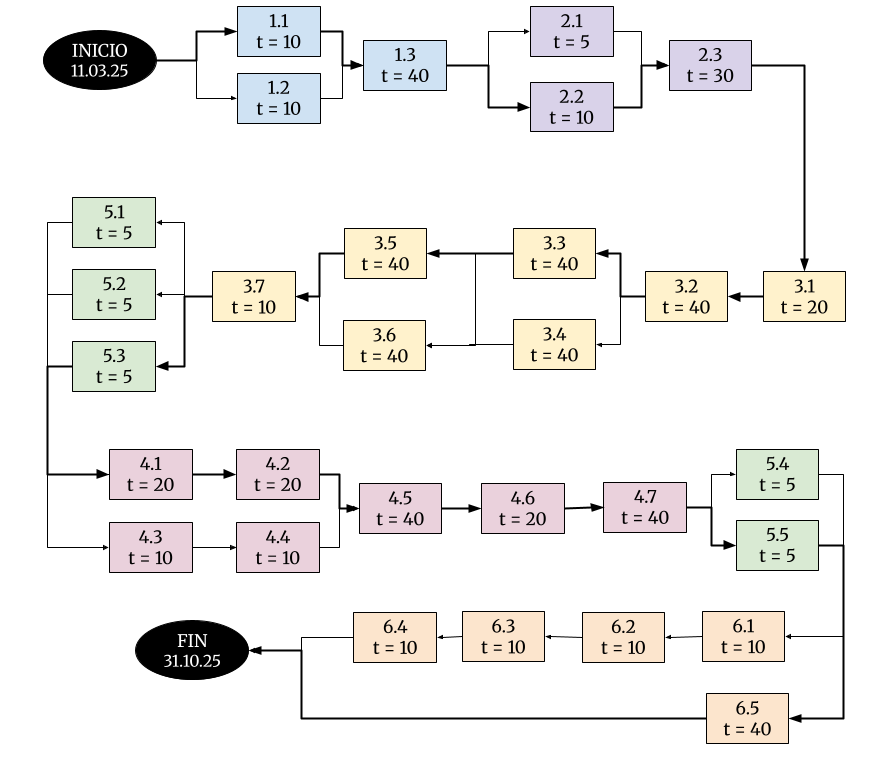
\includegraphics[width=.85\textwidth]{./Figuras/Diagrama-AoN.png}
\caption{Diagrama de \textit{Activity on Node}.}
\label{fig:AoN}
\end{figure}


\section{11. Diagrama de Gantt}
\label{sec:gantt}

En la figura \ref{fig:diagGantt} se presenta el diagrama de Gantt, elaborado a partir del desglose de tareas y del diagrama AoN definido en el punto anterior. Considerando la paralelización de tareas establecida, el diagrama muestra la fecha estimada de inicio y finalización de cada actividad, tomando en cuenta su duración y asumiendo una dedicación promedio de 20 horas semanales al desarrollo del proyecto.

Al igual que en el diagrama AoN, cada grupo de tareas está representado con un color diferente para facilitar su identificación. El proyecto tiene como fecha de inicio el 11 de marzo de 2025 y finalizará la semana del 14 de octubre de 2025.


\begin{figure}[htpb]
\centering 
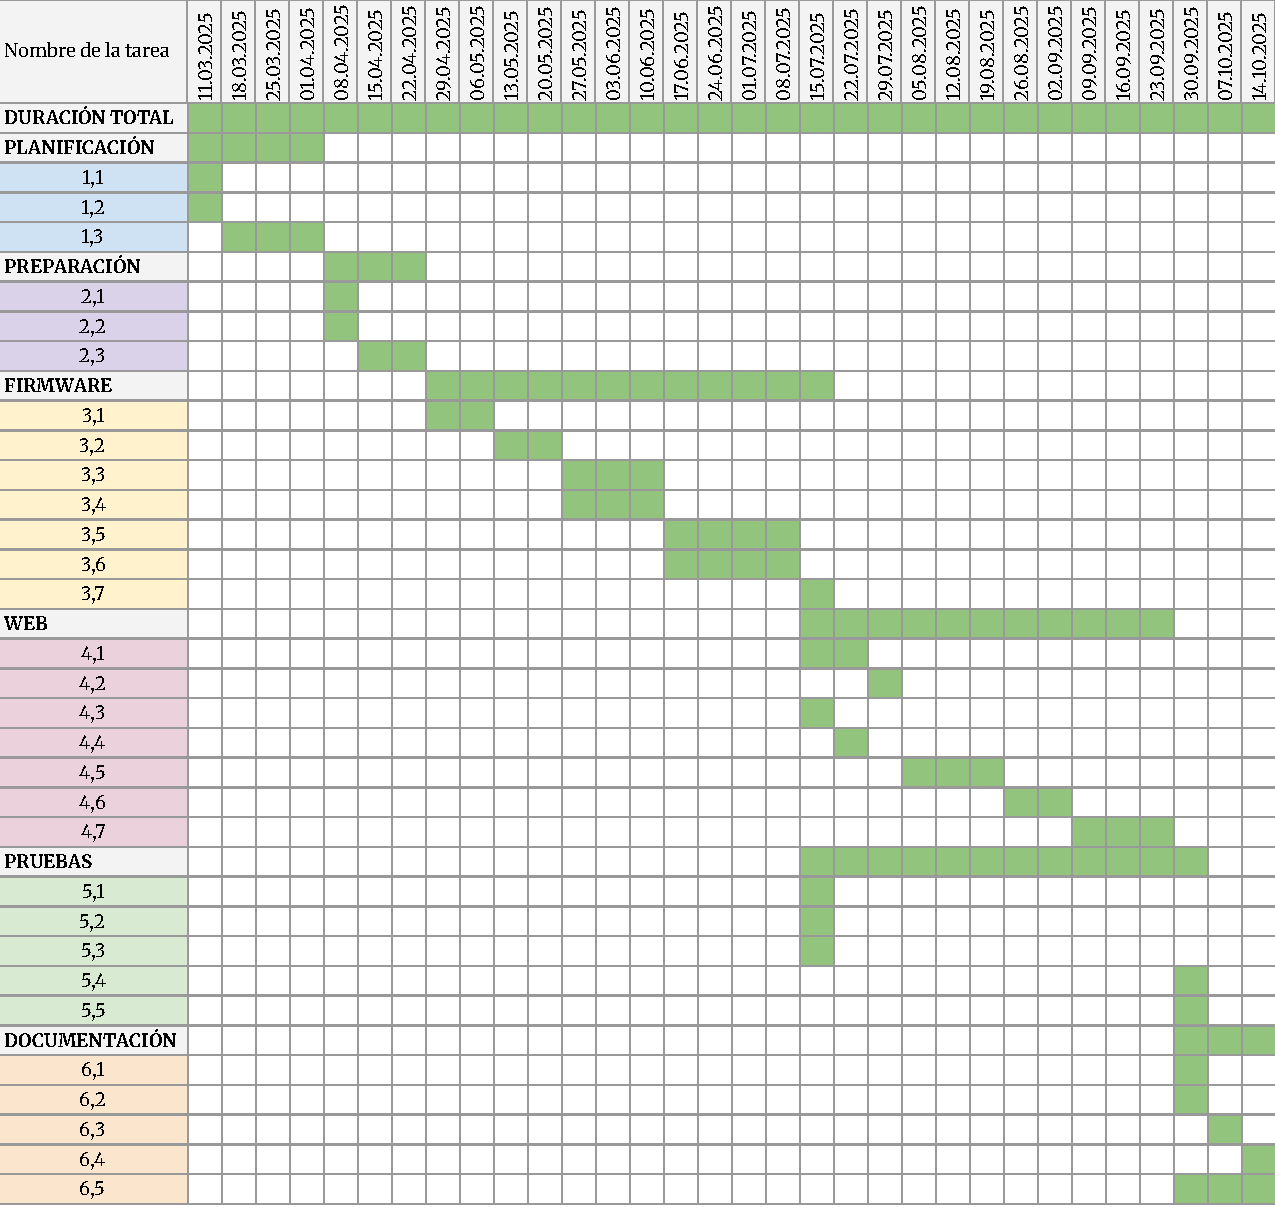
\includegraphics[height=.62\textheight]{./Figuras/Gantt.pdf}
\caption{Diagrama de Gantt.}
\label{fig:diagGantt}
\end{figure}


\section{12. Presupuesto detallado del proyecto}
\label{sec:presupuesto}

A continuación se presenta la tabla de costos directos e indirectos asociados a este proyecto. Los valores unitarios se encuentran expresados en dolares estadounidenses (USD). Los valores totales se encuentran en USD y en pesos argentinos (ARS). 

Tasa de conversion: USD \$1 = ARS \$1072.87, correspondiente a la fecha 2 de abril de 2025.

\begin{table}[htpb]
\centering
\begin{tabularx}{\linewidth}{@{}|X|c|r|r|@{}}
\hline
\rowcolor[HTML]{C0C0C0} 
\multicolumn{4}{|c|}{\cellcolor[HTML]{C0C0C0}COSTOS DIRECTOS} \\ \hline
\rowcolor[HTML]{C0C0C0} 
Descripción &
  \multicolumn{1}{c|}{\cellcolor[HTML]{C0C0C0}Cantidad} &
  \multicolumn{1}{c|}{\cellcolor[HTML]{C0C0C0}Valor unitario} &
  \multicolumn{1}{c|}{\cellcolor[HTML]{C0C0C0}Valor total} \\ \hline 

  \multicolumn{1}{|l|}{Módulos ESP32-C3 mini} &
  \multicolumn{1}{c|}{4} &
  \multicolumn{1}{c|}{\$6} &
  \multicolumn{1}{c|}{\$24} \\ \hline
 
  \multicolumn{1}{|l|}{Componentes electrónicos adicionales} & 
  \multicolumn{1}{c|}{1} &
  \multicolumn{1}{c|}{\$10} &
  \multicolumn{1}{c|}{\$10} \\ \hline

  \multicolumn{1}{|l|}{Computadora personal} & 
  \multicolumn{1}{c|}{1} &
  \multicolumn{1}{c|}{\$400} &
  \multicolumn{1}{c|}{\$400} \\ \hline
  
  \multicolumn{1}{|l|}{Hora de trabajo ingeniera} & 
  \multicolumn{1}{c|}{600} &
  \multicolumn{1}{c|}{\$10} &
  \multicolumn{1}{c|}{\$6000} \\ \hline
 
  \multicolumn{1}{|l|}{Hora de consultoria especialista} & 
  \multicolumn{1}{c|}{14} &
  \multicolumn{1}{c|}{\$20} &
  \multicolumn{1}{c|}{\$280} \\ \hline
  
\multicolumn{3}{|c|}{SUBTOTAL EN USD} &
  \multicolumn{1}{c|}{\$6714} \\ \hline
 
 \multicolumn{3}{|c|}{SUBTOTAL EN ARS} &
  \multicolumn{1}{c|}{\$7'203.249} \\ \hline
  
\rowcolor[HTML]{C0C0C0}

\multicolumn{4}{|c|}{\cellcolor[HTML]{C0C0C0}COSTOS INDIRECTOS} \\ \hline
\rowcolor[HTML]{C0C0C0} 
Descripción &
  \multicolumn{1}{c|}{\cellcolor[HTML]{C0C0C0}Cantidad} &
  \multicolumn{1}{c|}{\cellcolor[HTML]{C0C0C0}Valor unitario} &
  \multicolumn{1}{c|}{\cellcolor[HTML]{C0C0C0}Valor total} \\ \hline

  \multicolumn{1}{|l|}{Servicios de oficina mensual} & 
  \multicolumn{1}{c|}{7} &
  \multicolumn{1}{c|}{\$25} &
  \multicolumn{1}{c|}{\$175} \\ \hline
  
  \multicolumn{1}{|l|}{Fondo de riesgos para ESP32-C3} & 
  \multicolumn{1}{c|}{2} &
  \multicolumn{1}{c|}{\$6} &
  \multicolumn{1}{c|}{\$12} \\ \hline
    
  \multicolumn{3}{|c|}{SUBTOTAL EN USD} &
  \multicolumn{1}{c|}{\$187} \\ \hline
  
  \multicolumn{3}{|c|}{SUBTOTAL EN ARS} &
  \multicolumn{1}{c|}{\$200.625} \\ \hline
  
\rowcolor[HTML]{C0C0C0}
\multicolumn{3}{|c|}{TOTAL EN USD} &
\multicolumn{1}{c|}{\$6901} \\ \hline
  
\rowcolor[HTML]{C0C0C0}
\multicolumn{3}{|c|}{TOTAL EN ARS} &
\multicolumn{1}{c|}{\$7'403.848} \\ \hline

\end{tabularx}%
\end{table}




\section{13. Gestión de riesgos}
\label{sec:riesgos}

\begin{consigna}{red}
a) Identificación de los riesgos (al menos cinco) y estimación de sus consecuencias:
 
Riesgo 1: detallar el riesgo (riesgo es algo que si ocurre altera los planes previstos de forma negativa)
\begin{itemize}
	\item Severidad (S): mientras más severo, más alto es el número (usar números del 1 al 10).\\
	Justificar el motivo por el cual se asigna determinado número de severidad (S).
	\item Probabilidad de ocurrencia (O): mientras más probable, más alto es el número (usar del 1 al 10).\\
	Justificar el motivo por el cual se asigna determinado número de (O). 
\end{itemize}   

Riesgo 2:
\begin{itemize}
	\item Severidad (S): X.\\
	Justificación...
	\item Ocurrencia (O): Y.\\
	Justificación...
\end{itemize}

Riesgo 3:
\begin{itemize}
	\item Severidad (S):  X.\\
	Justificación...
	\item Ocurrencia (O): Y.\\
	Justificación...
\end{itemize}


b) Tabla de gestión de riesgos:      (El RPN se calcula como RPN=SxO)

\begin{table}[htpb]
\centering
\begin{tabularx}{\linewidth}{@{}|X|c|c|c|c|c|c|@{}}
\hline
\rowcolor[HTML]{C0C0C0} 
Riesgo & S & O & RPN & S* & O* & RPN* \\ \hline
       &   &   &     &    &    &      \\ \hline
       &   &   &     &    &    &      \\ \hline
       &   &   &     &    &    &      \\ \hline
       &   &   &     &    &    &      \\ \hline
       &   &   &     &    &    &      \\ \hline
\end{tabularx}%
\end{table}

Criterio adoptado: 

Se tomarán medidas de mitigación en los riesgos cuyos números de RPN sean mayores a...

Nota: los valores marcados con (*) en la tabla corresponden luego de haber aplicado la mitigación.

c) Plan de mitigación de los riesgos que originalmente excedían el RPN máximo establecido:
 
Riesgo 1: plan de mitigación (si por el RPN fuera necesario elaborar un plan de mitigación).
  Nueva asignación de S y O, con su respectiva justificación:
  \begin{itemize}
	\item Severidad (S*): mientras más severo, más alto es el número (usar números del 1 al 10).
          Justificar el motivo por el cual se asigna determinado número de severidad (S).
	\item Probabilidad de ocurrencia (O*): mientras más probable, más alto es el número (usar del 1 al 10).
          Justificar el motivo por el cual se asigna determinado número de (O).
	\end{itemize}

Riesgo 2: plan de mitigación (si por el RPN fuera necesario elaborar un plan de mitigación).
 
Riesgo 3: plan de mitigación (si por el RPN fuera necesario elaborar un plan de mitigación).

\end{consigna}


\section{14. Gestión de la calidad}
\label{sec:calidad}

\begin{consigna}{red}
Elija al menos diez requerimientos que a su criterio sean los más importantes/críticos/que aportan más valor y para cada uno de ellos indique las acciones de verificación y validación que permitan asegurar su cumplimiento.

\begin{itemize} 
\item Req \#1: copiar acá el requerimiento con su correspondiente número.

\begin{itemize}
	\item Verificación para confirmar si se cumplió con lo requerido antes de mostrar el sistema al cliente. Detallar.
	\item Validación con el cliente para confirmar que está de acuerdo en que se cumplió con lo requerido. Detallar. 
\end{itemize}

\end{itemize}

Tener en cuenta que en este contexto se pueden mencionar simulaciones, cálculos, revisión de hojas de datos, consulta con expertos, mediciones, etc.  

Las acciones de verificación suelen considerar al entregable como ``caja blanca'', es decir se conoce en profundidad su funcionamiento interno.  

En cambio, las acciones de validación suelen considerar al entregable como ``caja negra'', es decir, que no se conocen los detalles de su funcionamiento interno.

\end{consigna}

\section{15. Procesos de cierre}    
\label{sec:cierre}

\begin{consigna}{red}
Establecer las pautas de trabajo para realizar una reunión final de evaluación del proyecto, tal que contemple las siguientes actividades:

\begin{itemize}
	\item Pautas de trabajo que se seguirán para analizar si se respetó el Plan de Proyecto original:\\
	 - Indicar quién se ocupará de hacer esto y cuál será el procedimiento a aplicar. 
	\item Identificación de las técnicas y procedimientos útiles e inútiles que se emplearon, los problemas que surgieron y cómo se solucionaron:\\
	 - Indicar quién se ocupará de hacer esto y cuál será el procedimiento para dejar registro.
	\item Indicar quién organizará el acto de agradecimiento a todos los interesados, y en especial al equipo de trabajo y colaboradores:\\
	  - Indicar esto y quién financiará los gastos correspondientes.
\end{itemize}

\end{consigna}

\end{document}